% "pdf"

\documentclass[a4paper,12pt]{article}

\usepackage[french]{babel}
\usepackage[T1]{fontenc}
\usepackage[utf8x]{inputenc}

\usepackage[margin=2cm]{geometry}
\usepackage{pifont}

\usepackage[colorlinks=true,
            linkcolor=black]{hyperref}
\usepackage{titletoc}
\usepackage{titlesec}

\usepackage{soul}
% \usepackage{ulem}

\usepackage[french, lined,ruled]{algorithm2e}

\title{\Huge\textbf{Rapport de Phase 2 du Groupe 1}}
\author{Shimi Adam \& Megna Anaël \& Lemarchand Benoît}
\date{Vendredi, 29 Mai 2015}

\usepackage{fancyhdr}
\pagestyle{fancy}
\renewcommand{\headrulewidth}{0pt}
\lfoot{} \cfoot{} \rfoot{\thepage} \lhead{} \chead{} \rhead{}

\usepackage{amsmath}
\usepackage{amssymb}
\usepackage{amsthm}
\usepackage{mathtools}
\usepackage{mathrsfs}
\usepackage{stmaryrd}
\usepackage{esint}
\usepackage{esvect}
\usepackage{multirow}

\DeclareMathOperator{\Tr}{Tr}

\newtheorem*{remark}{Remarque}
\newtheorem*{erratum}{Erratum}

\usepackage{listings}

\newcommand{\norme}[1]{\left\Vert #1\right\Vert}

\renewcommand{\phi}{\varphi}
\renewcommand{\epsilon}{\varepsilon}

\setlength{\parindent}{1em}

\begin{document}

\begin{titlepage}
  \maketitle
  \thispagestyle{empty}
  \tableofcontents
\end{titlepage}

\section{Introduction}

    Nous arrivons à la fin de ce projet, et il est maintenant temps
    d'analyser le travail qui a été fait par notre groupe, à la fois
    pour présenter nos résultats, mais aussi pour pouvoir nous améliorer.

    Dans un premier temps, nous avons eu à implémenter deux méthodes
    d'analyse d'un modèle physique fourni (dérivée des \emph{Shallow Water
    Equations}) :

    \paragraph{}
    \begin{itemize}
        \item La reconstruction, qui consiste à partir de multiples itérations
        du modèle pour déduire le comportement de celui-ci pour des conditions
        initiales données.
        \item La classification, qui elle part aussi de multiples itérations
        du modèle, mais cette fois ci pour déduire un paramètre d'entrée de
        celui-ci.
    \end{itemize}

\bigskip

    Notre travail personnel dans la mise en place de ces deux méthodes
    a été principalement d'implémenter un algorithme efficace de calcul
    des valeurs singulières et de choisir une méthode itérative pour la
    reconstruction.

    En ce qui concerne l'algorithme pour la décomposition en valeurs
    singulières, il sera explicité dans la section suivante.

    Quand à la méthode itérative que nous avons utilisée pour
    déterminer $\alpha$ dans la reconstruction, il s'agit d'une
    \emph{steepest descent} sur l'équation normale $U_{0}^t*U_{0}*\alpha = U_{0}^t*Z_0$.

      \begin{erratum}Nous avons utilisé la \emph{steepest descent} dans
    cette phase 1, alors que le critère d'arrêt sur la recherche
    des valeurs propres assure dans l'immense majorité des cas
    que toutes les valeurs singulières de U sont positives, et
    donc que $U0^T*U0$ est inversible.

    Nous pouvions donc directement résoudre l'équation normale
    (comme cela a été fait dans la correction).

    Nous nous excusons encore une fois pour cette erreur stupide.
    \end{erratum}

    \paragraph{}
    Dans un second temps, nous avons du implémenter la \emph{subspace Iteration
    Method} en fortran, pour accélérer celle-ci, puis l'interfacer avec
    \emph{Matlab}.

    Enfin, nous avons conduit quelques tests sur ces implémentations,
    ainsi que d'autres sur une modification liée au modèle physique.

\newpage

\section{Implémentation de la \emph{Subspace Iteration Method} en Fortran}

    Tout d'abord, nous rappelons le pseudo code fourni dans le compte-rendu
    de la phase 1, avant d'expliquer l'algorithme en lui-même, ainsi que
    de préciser l'implémentation en Fortran.

    \paragraph{}
    \begin{algorithm}[H]
    \DontPrintSemicolon
    $V = matrice\ orthogonale\ quelconque \in \mathbb{R}^{m*l}$\;
    $niter = 0$\;
    $converged = 0$\;
    $PercentReached = 0$\;
    $normeA = \norme{Z^T*Z}$\;
    \Repeat{$PercentReached \leq PercentInfo$ or $niter < MaxIter$}{
       \For{$i=1, p$}{
            $V = Z^T*Y$\;
            $V = Z*Y$\;
        }
        $V = \mathrm{Gram-Schmidt}(V)\footnote{Nous ne rappellons pas l'algorithme d'orthogonalisation de Gram-Schmidt, mais celui-çi est implémenté dans le code}$\;
        $H = Z^T*V$\;
        $H = H^T*H$\;
        $[X,\Lambda] = decomposition\ spectrale\ de\ H$\;
        $[X,\Lambda] = ordonnancement\ decroissant\ de\ [X,\Lambda]$\;
        $V = V*X$\;
        \For {$i=converged + 1, n$}{
            \eIf{$\displaystyle \frac{\norme{Z*Z^T*V(i) - \Lambda(i,i).V(i)}}{normeA} \leq \epsilon$}{
                $converged = converged + 1$\;
                $\displaystyle PercentReached = 1 - \frac{\norme{Z - \sum\limits_{j=1}^i \sqrt[4]{\Lambda(i,i)}V(i)V(i)^TZ^T}}{\sqrt{normeA}}$\;
            } {
                break\;
            }
        }
        $niter = niter + 1$\;
    }
    \caption{Méthode du sous-espace singulier dominant}
    \end{algorithm}

\newpage

    \paragraph{}
    Il est temps d'expliquer plus précisément cet algorithme. Comme
    expliqué dans le sujet de la phase 1, il est adapté de la \emph{power
    method}, qui permet de calculer une à une les valeurs propres dans
    l'ordre décroissant d'une matrice carrée.

    \paragraph{}
    Comme dans l'algorithme de la \emph{power method}, le but est ici de
    polariser des vecteurs selon les vecteurs propres en les multipliant
    par la matrice, afin de les faire tendre vers les dits vecteurs propres
    après suffisamment d'itérations. Les principales différences ici étant
    que nous travaillons sur toutes les valeurs propres en parallèle (la
    raison pour laquelle notre algorithme peut renvoyer la proportion demandée
    de valeurs propres en une itération, alors que la \emph{power method} prendrait
    dans le meilleur des cas la somme des multiplicités de ces valeurs propres).

    Une autre différence facilement traitable est le fait que nous cherchons ici
    les valeurs singulières et les vecteurs singuliers gauche d'une matrice
    rectangle. Il suffit de remarquer que ce sont les valeurs propres et les
    vecteurs propres de la matrice consistant en le produit de notre
    matrice rectangulaire avec sa transposée pour se ramener au cas carré.

    \paragraph{}
    Comme dit plus haut, la \emph{subspace method} consiste à polariser non pas
    un vecteur selon la valeur propre dominante, mais une base de $n$ vecteurs
    orthogonaux selon les $n$ valeurs propres dominantes. Pour cela, la méthode
    est la même que dans la \emph{power method}, c'est à dire une multiplication par
    la matrice carré dont on cherche les valeurs propres. A noter qu'il est
    possible de multiplier plusieurs fois la base par cette matrice à chaque
    itération, pour s'assurer que tous les vecteurs ne sont pas polarisés par
    la valeur propre dominante.

    Enfin on orthogonalise après coup les vecteurs par Gram-Schmidt,
    afin de laisser à chaque vecteur \og approximé \fg une polarisation selon un unique vecteur
    propre.

    \paragraph{}
    Ensuite, extraire les approximations de vecteurs propres que sont devenus
    les vecteurs de la base orthonormale s'avère un peu plus dur que dans la
    \emph{power method}, étant donné qu'ils sont \og enfouis \fg dans ces vecteurs.

    L'idée est d'exprimer les vecteurs de cette base orthonormale dans la
    base de vecteurs propres de la matrice carrée. Nous
    allons recourir aux notations de l'énoncé, c'est-à-dire que la matrice
    carrée dont nous cherchons les valeurs et vecteurs propres est notée $A$
    et que la matrice contenant la base des vecteurs orthogonaux polarisés
    par $A$ puis orthogonalisés de nouveau est notée $V$. Ainsi, nous calculons
    la matrice $V^T*A*V$, aussi connue sous le nom de quotient de Rayleigh de
    la base $V$ par la matrice $A$.

    Puis, nous calculons les valeurs propres et les vecteurs propres du quotient
    de Rayleigh. En faisant le simple calcul $V*V^T*A*V*V^T = A$, on voit qu'il
    suffit de réexprimer les vecteurs propres du quotient de Rayleigh dans la base
    de $V$ (par une multiplication matricielle donc) pour obtenir une approximation
    des vecteurs propres de $A$

    \paragraph{}
    Enfin, pour décider si un couple valeur et vecteur propre est suffisamment proche
    pour être accepté, nous calculons l'erreur du vecteur propre par la multiplication
    par $A$, rescalée par la norme de A pour être indépendante de la valeur de la
    valeur propre considérée. Plus formellement, si $\lambda_i$ $v(:,i)$ sont
    respectivement la valeur propre et le vecteur propre approximé, nous calculons
    $\frac{\norme{A*v(:,i) - \lambda_i*v(:,i)}}{\norme{A}}$ et nous le comparons
    à l'erreur acceptée.

    \bigskip
    \paragraph{}
    En ce qui concerne l'implémentation en fortran à proprement parler, il a surtout
    fallut déconstruire les calculs matriciels et vectoriels complexes en séquences
    de primitives.

    Aussi, nous avons rendu explicite les astuces utilisées dans la partie 1 pour
    éviter de calculer la matrice $A$, étant donné que dans le cas qui nous intéresse
    , celle-ci cause un \emph{memory overflow}.

\newpage
\section{Test de l'implémentation Fortran}

    \paragraph{}
    Dans cette partie, il s'agit d'analyser les résultats des comparaisons
    entre le temps mis par notre implémentation fortran, la même implémentation
    en version matrice symétrique (c'est-à-dire avec le calcul explicite de la
    matrice $A = Z*Z^T$) et la méthode dédiée de LAPACK, fortement optimisée
    par des années de recherche.

    \paragraph{}
    Tout d'abord, nous avons remarqué que la comparaison qui faisait le plus sens
    était celle de notre implémentation et de LAPACK. En effet, la version symétrique,
    en plus d'être la version de notre algorithme inapplicable à notre problème de départ
    , ne dévie de notre implémentation que par un facteur constant, le quotient du temps
    mis pour faire deux multiplications matricielle par le temps mis pour faire une seule
    multiplication matricielle, mais par le produit des deux matrices précédentes.

    \paragraph{}
    Ensuite, il y a la question de quels paramètres faire varier. $p$ est un choix
    inévitable, étant donné que nous ne le faisons pas varier dans les tests du matlab.
    Pour avoir une nappe en trois dimensions, il manque une variable, que nous
    posons comme $n$.

    En effet, fixer $m$ fait sens, étant donné que c'est ce qu'il se passera dans le
    problème où la méthode sera utilisée. La taille du sous-espace invariant de même.

    Enfin, on refait les tests pour les 4 valeurs d'imat, afin de généraliser les
    résultats.

    \bigskip
    \begin{center}
    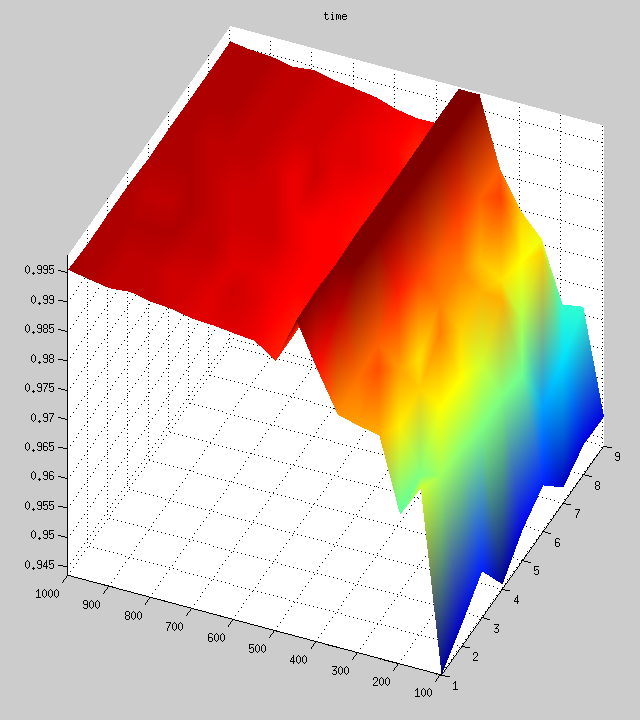
\includegraphics[width=20em, height=20em]{imat1.png}
    \end{center}

    \bigskip
    \begin{center}
    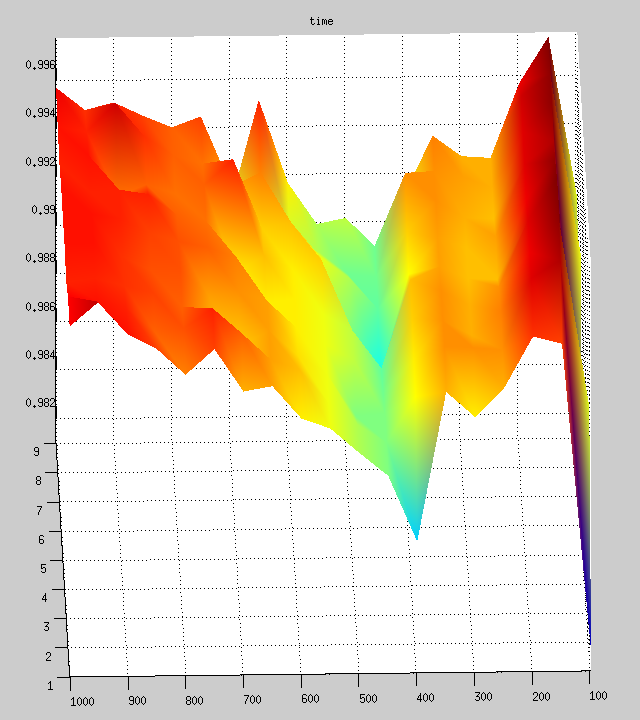
\includegraphics[width=20em, height=20em]{imat2.png}
    \end{center}

    \begin{center}
    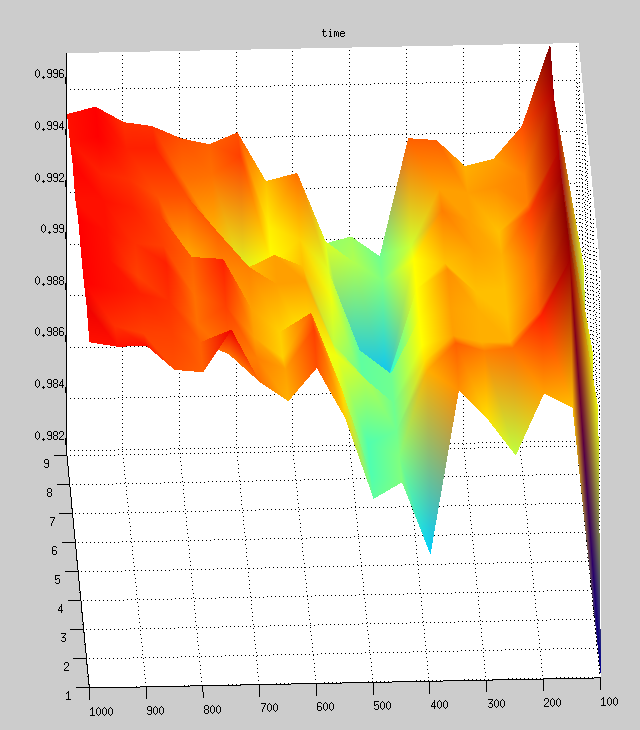
\includegraphics[width=20em, height=20em]{imat3.png}
    \end{center}

    \begin{center}
    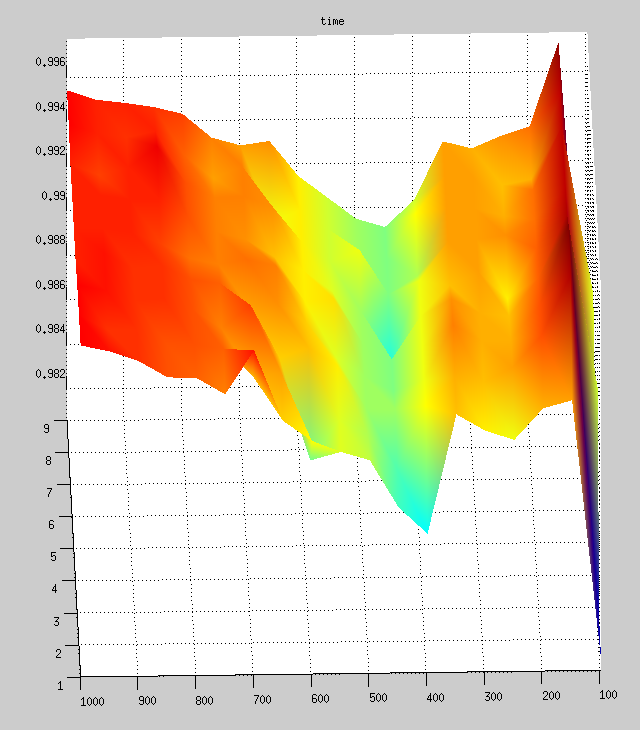
\includegraphics[width=20em, height=20em]{imat4.png}
    \end{center}

    \paragraph{}
    Nous remarquons que les résultats avec les générateurs de matrice 2,3 et 4
    sont assez similaires, alors que les résultats obtenus à l'aide du générateur
    de matrice 1 sont plus lisses. Nous choisissons de nous attarder sur les résultats
    pour $imat = 4$, la nappe la plus lisse des trois nappes les plus générales.

    \paragraph{}
    En ce qui concerne l'interprétation des résultats, nous allons le faire en deux temps.

    \bigskip

    \paragraph{}
    Premièrement, les variations en fonction de $n$ expriment comment les générateurs
    de matrice répartissent les valeurs singulières. En effet, la principale raison pour
    laquelle notre routine est plus lente que celle de LAPACK est dans un cas où
    il faut calculer beaucoup de valeurs singulières, et donc où l'aspect itératif
    montre ses limites.

    \paragraph{}
    Dans un second temps, les variations en fonction de $p$ indiquent une notion
    assez intéressante, qui est celle de l'équilibre dans la répartition des
    valeurs singulières.

    En effet, plus $p$ est grand, plus il augmente le temps
    que prend une itération de la routine, étant donné qu'il augmente le nombre
    de produits matriciels.

    Mais, pour certaines valeurs de $p$, plus de valeurs singulières peuvent
    converger en même temps, ce qui baisse le nombre d'itérations de la routine.

    Comme nous le verrons dans la suite du rapport, adapter $p$ à la matrice est
    le genre d'amélioration dont notre routine a besoin.

\newpage
\section{Test de l'implémentation Matlab}

    \paragraph{}
    Les tests que nous avons mis en place pour comparer l'efficacité en temps et
    en précision de notre implémentation fortran face à la $svd$ consiste, à l'image
    de ceux de la section précédente, au calcul, pour la même matrice, de l'erreur
    relative et du temps relatif par rapport à la $svd$.

    En ce qui concerne les paramètres variant, nous avons considéré qu'il était
    acceptable de prendre $p$ fixe, étant donne que l'utilité d'un $p$ différent de 1
    dans certains cas a été étudié dans les expériences précédentes.

    De plus, cela nous permet de construire des nappes de résultats en trois dimensions,
    selon $Nens$ et $percentInfo$.

    \bigskip
    \begin{center}
    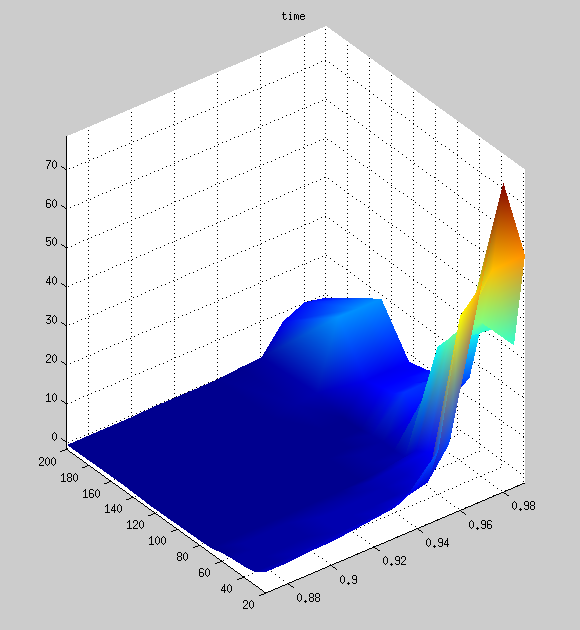
\includegraphics[width=20em, height=20em]{time1.png}
    \end{center}

    \paragraph{}
    Une première observation sur ce graphique est que dans la grande majorité
    des cas traités, la nappe reste relativement proche du plan $z=0$. Cela
    nous indique que si notre implémentation ne bat presque jamais la $svd$
    de matlab, il lui arrive de l'égaler.

    Bien sûr, ce qui nous intéresse vraiment concerne les valeurs des paramètres
    pour lesquels notre fonction va clairement moins vite que $svd$.

    Nous pouvons remarquer en premier lieu que plus $Nens$ est faible, à
    $percentInfo$
    fixé, plus la $svd$ gagne du terrain. Cela s'explique par le fait que réduire
    $Nens$ revient à réduire le nombre de valeurs singulières, donc à avoir soit des
    valeurs singulières plus proches, auquel cas notre méthode aura du mal à
    converger pour toutes les valeurs singulières nous intéressant, soit à devoir
    prendre une grosse majorité des valeurs singulières (surtout que nous testons
    avec des $percentInfo$ élevés), auquel cas notre algorithme aux multiples itérations
    se fait évidemment battre par un algorithme qui calcule toutes les valeurs
    singulières d'un coup.

    \bigskip
    \begin{center}
    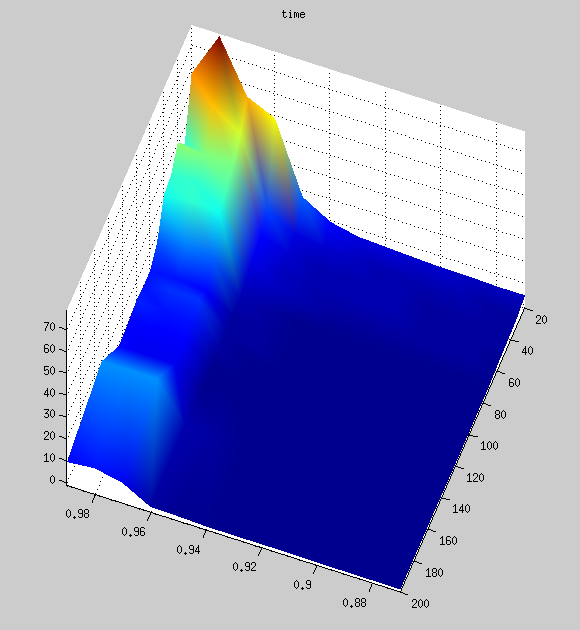
\includegraphics[width=20em, height=20em]{time2.png}
    \end{center}

    \paragraph{}
    Cet angle nous montre maintenant que la précision à partir de laquelle la $svd$
    surpasse largement notre algorithme est $0.96$. Cela fait sens qu'un trop grand
    $percentInfo$ nous pose des soucis, étant donné que l'on retombe dans ce cas
    dans le problème de la majorité des valeurs singulières : il n'y a pas
    d'intérêt à les calculer séparément si nous les voulons toutes.

    \bigskip
    \begin{center}
    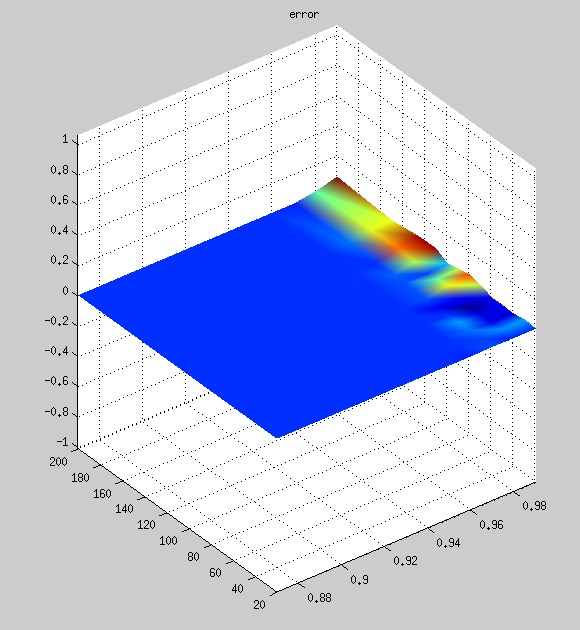
\includegraphics[width=20em, height=20em]{error.png}
    \end{center}

    \paragraph{}
    Enfin, l'erreur relative est très proche de zéro, même aux extrêmes du graphe.
    Ainsi, notre implémentation, à défaut d'être toujours rapide, est presque toujours
    précise.

    Nous remarquons tout de même que l'erreur relative augmente légèrement pour de
    grands $Nens$ et $percentInfo$.

\newpage
\section{Addendum : prise en compte du modèle physique}

    \paragraph{}
    Une fois l'implémentation en fortran et les comparaisons avec $svd$ faites,
    nous avons voulu voir si nous pouvions aller plus vite que matlab. Évidemment,
    pour une matrice quelconque, ce désir est assez illusoire.

    Mais nous avons un avantage par rapport à matlab en ce qui concerne les
    matrices sur lesquelles nous travaillons : nous savons qu'elles découlent
    d'un modèle physique, et donc nous avons une information de premier choix
    sur la manière dont les coefficients de cette matrice sont corrélés.

    L'idée derrière notre amélioration est d'échantillonner à nouveau toutes les
    colonnes de $Z$, en considérant, comme indiquée par les équations différentielles
    du modèle, que $z(.,.,t)$ est dérivable au voisinage de tout point $x,y$ de la grille.
    Ainsi, chaque point de la grille observé à l'instant t contient dans son $z$ des
    informations sur ses voisins.

    D'où l'hypothèse que prendre un coefficient de chaque colonne de Z sur trois suffit
    à nous donner les informations nécessaires, tout en réduisant la taille de la
    matrice à traiter.

    Nous échantillonnons $Z$ de cette manière avant de la fournir à notre méthode
    fortran, puis nous reconstruisons une $U$ de la bonne taille en remplissant une
    matrice du format de $Z$, remplie de zéros, par les lignes de $U$, toutes les trois
    lignes.

    Voici les résultats :

    \bigskip
    \begin{center}
    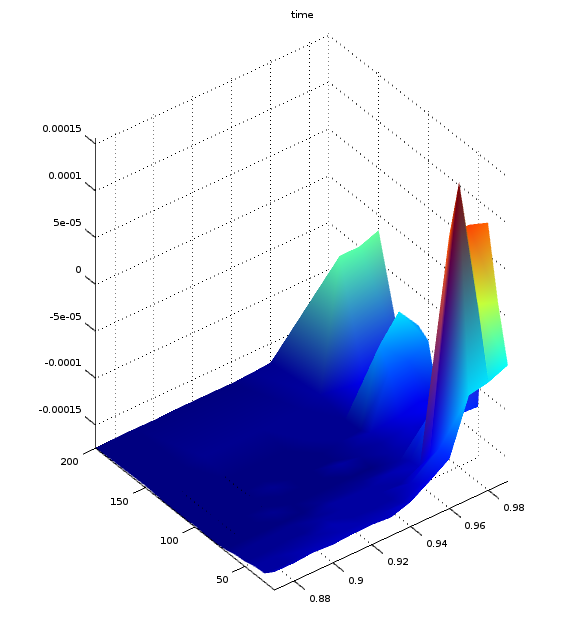
\includegraphics[width=20em, height=20em]{time2_1.png}
    \end{center}

    \paragraph{}
    Tout de suite, nous remarquons que cette nappe a la même forme que celle de
    notre méthode non modifiée, si ce n'est l'homothétie qui rend cette nappe ci
    majoritairement négative.

    Cela signifie donc que dans la vaste majorité des cas, cette méthode est plus
    rapide, voir significativement plus rapide que la $svd$.

    Cependant, tout ça n'a d'intérêt que si l'erreur reste acceptable.

    \bigskip
    \begin{center}
    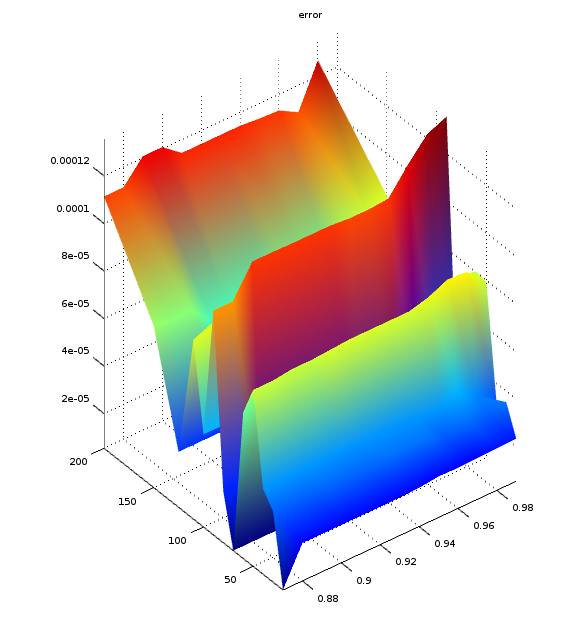
\includegraphics[width=20em, height=20em]{error2_1.png}
    \end{center}

    Clairement, l'erreur relative est plus importante que pour notre méthode
    classique, mais si l'on regarde l'axe vertical, on remarque qu'elle reste
    très faible, bien que positive.

    Un autre point intéressant est l'aspect de cette nappe d'erreur, avec une
    sorte d'oscillation selon l'axe des $Nens$. Pour l'instant, nous n'avons pas
    pu expliquer cet aspect.

    Au final, l'idée d'échantillonner en tenant compte du modèle physique permet
    de gagner un temps significatif, tout en ayant une erreur relative très
    faible. Peut-être une piste à creuser.

\newpage
\section{Conclusions}

    \paragraph{}
    Après avoir travaillé dessus durant tout un projet, la méthode du \emph{subspace
    iteration} nous semble à la fois puissante et adaptée à la situation, avec
    un bémol toutefois : la fixité de $p$.

    Il manque vraiment à cette méthode un moyen de trouver le $p$ "optimal"
    pour une matrice donnée, ce qui permettrait de \og poncer \fg en grande partie
    les pics du temps relatif par rapport à la $svd$.

    \paragraph{}
    En ce qui concerne le projet en général, il a eu le mérite de nous montrer
    une véritable application des techniques d'ALN, et de nous introduire à ce
    point de vue vectoriel et matriciel sur le monde physique, rempli de sous
    espaces significatifs et de polarisations selon une base.

\end{document}
